\documentclass[tikz,border=6pt]{standalone}
\usepackage{xcolor}
\usepackage{pgfplots}
\pgfplotsset{compat=1.18}

\definecolor{lineblue}{HTML}{4A90D9}

\begin{document}
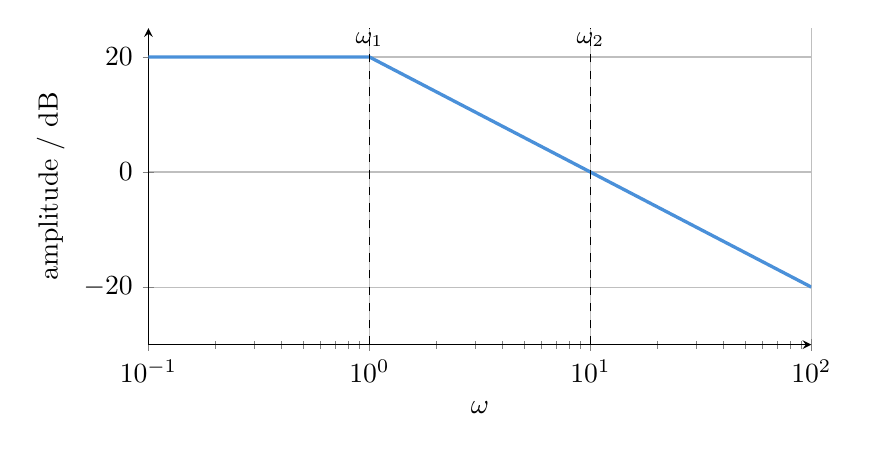
\begin{tikzpicture}
  \begin{axis}[
    width=10cm,
    height=5.6cm,
    xmode=log,
    xmin=0.1, xmax=100,
    ymin=-30, ymax=25,
    axis lines=left,
    xlabel={$\omega$},
    ylabel={amplitude / dB},
    xtick={0.1,1,10,100},
    xticklabels={$10^{-1}$,$10^0$,$10^1$,$10^2$},
    ytick={-20,0,20},
    grid=major
  ]
    \addplot[lineblue, line width=1.2pt] coordinates {(0.1,20) (1,20) (10,0) (100,-20)};
    \draw[dashed] (axis cs:1,-30) -- (axis cs:1,25);
    \draw[dashed] (axis cs:10,-30) -- (axis cs:10,25);
    \node at (axis cs:1,23) {\small $\omega_1$};
    \node at (axis cs:10,23) {\small $\omega_2$};
  \end{axis}
\end{tikzpicture}
\end{document}
